% -*- mode: noweb; noweb-default-code-mode: R-mode; -*-
%\VignetteIndexEntry{GeneAnswers}
%\VignetteKeywords{GeneAnswers, genelist, Microarray preprocessing}
%\VignetteDepends{GeneAnswers, annotate, igraph, AnnotationDbi, GO.db, KEGG.db, biomaRt, RCurl, XML}
%\VignettePackage{GeneAnswers}

\documentclass[a4paper]{article}

\usepackage{amsmath,pstricks}
\usepackage{hyperref}
\usepackage[authoryear,round]{natbib}

\newcommand{\Rfunction}[1]{{\texttt{#1}}}
\newcommand{\Robject}[1]{{\texttt{#1}}}
\newcommand{\Rpackage}[1]{{\textit{#1}}}
\newcommand{\Rclass}[1]{{\textit{#1}}}
\newcommand{\Rmethod}[1]{{\textit{#1}}}



\author{Gang Feng$^\ddagger$\footnote{g-feng (at) northwestern.edu}, Pan Du$^\ddagger$\footnote{dupan (at) northwestern.edu}, Warren A. Kibbe$^\ddagger$\footnote{wakibbe (at) northwestern.edu}, Simon Lin$^\ddagger$\footnote{s-lin2 (at) northwestern.edu}}
\usepackage{Sweave}
\begin{document}

\setkeys{Gin}{width=1\textwidth} 

\title{GeneAnswers, Integrated Interpretation of Genes }
\maketitle
\begin{center}$^\ddagger$Northwestern University Biomedical Informatics Center \\ Northwestern University, Chicago, IL, 60611, USA
\end{center}

\tableofcontents
%%%%%%%%%%%%%%%%%%%%%%%%%%%%%%%%%%%%%%%%%%%%%%

\section{Overview of GeneAnswers}
Microarray techniques have been widely employed in genomic scale studies for more than one decade. The standard analysis of microarray data is to filter out a group of genes from thousands of probes by certain statistical criteria. These genes are usually called significantly differentially expressed genes. Recently, next generation sequencing (NGS) is gradually adopted to explore gene transcription, methylation, etc. Also a gene list can be obtained by NGS preliminary data analysis. However, this type of information is not enough to understand the potential linkage between identified genes and interested functions. The integrated functional and pathway analysis with gene expression data would be very helpful for researchers to interpret the relationship between the identified genes and proposed biological or medical functions and pathways.

The \Rpackage{GeneAnswers} package provides an integrated solution for a group of genes and specified categories (biological or medical functions, such as Gene Ontology, Disease Ontology, KEGG, etc) to reveal the potential relationship between them by means of statistical methods, and make user-friendly network visualization to interpret the results. Besides the package has a function to combine gene expression profile and category analysis together by outputting concept-gene cross tables, keywords query on NCBI Entrez Gene and application of human based Disease ontology analysis of given genes from other species can help people to understand or discover potential connection between genes and functions.

\section{Citation}
For the people using \Rpackage{GeneAnswers} package, please cite the following papers in your publications.

* For DOLite:

Du, P., Feng, G., Flatow, J., Song, J., Holko, M., Kibbe, W.A. and Lin, S.M., (2009) 'From disease ontology to disease-ontology lite: statistical methods to adapt a general-purpose ontology for the test of gene-ontology associations', Bioinformatics 25(12):i63-8


* For GeneAnswers:

Feng, G., Du, P., Krett, N.L., Tessel, M., Rosen, S., Kibbe, W.A., and Lin, S.M., (submitted) 'Bioconductor Methods to Visualize Gene-list Annotations', 

Thanks for your help!

\section{Installation of GeneAnswers package}
In order to install the \Rpackage{GeneAnswers} package, the user needs to first install R, some related Bioconductor packages. You can easily install them by the following codes.

\begin{Sinput} 
source("http://bioconductor.org/biocLite.R")
biocLite("GeneAnswers")
\end{Sinput}

For the users want to install the latest developing version of \Rpackage{GeneAnswers}, which can be downloaded from the developing section of Bioconductor website. Some additional packages might be required to be installed because of the update the Bioconductor. These packages can also be found from the developing section of Bioconductor website. You can also directly install the source packages from the Bioconductor website by specify the developing version number, which can be found at the Bioconductor website. Suppose the developing version is 2.5, to
install the latest \Rpackage{GeneAnswers} pakcage in the Bioconductor developing version, you can use the following command:

\begin{Sinput}
install.packages("GeneAnswers",repos="http://www.bioconductor.org/packages/2.5/bioc",type="source")
\end{Sinput} 

\section{Object models of major classes}
The \Rpackage{GeneAnswers} package has one major class: {\bf GeneAnswers}. It includes the following slots:

1. {\it geneInput}: a data frame containing gene Entrez IDs with or without any related values. The values could be foldChange, p value, or other values. These data can be used for concept-gene network. Genes with positive values will be represented as red nodes, while negative value genes are green nodes.

2. {\it testType}: statistical test method. Current version supports hypergeometric test to test relationship between genes and specified categories.

3. {\it pvalueT}: the cutoff of statistical test. Any categories will not be reported if the p value is more than the cutoff.

4. {\it genesInCategory}: a list containing genes belonging to categories. The names of the list are categories.

5. {\it geneExpProfile}: a data frame to store gene expression data. If not available, it could be NULL.

6. {\it annLib}: annotation database used for statistical test.

7. {\it categoryType}: functional or medical category used for statistical test.

8. {\it enrichmentInfo}: a data frame containing filtered categories with statistical results by specified pvalueT.

The figure, 'Flow chart of GeneAnswers', shows how \Rpackage{GeneAnswers} package works. A group of genes are essential. We use unique Entrez gene IDs to represent genes. Any relative feature values of these genes can also be optional input information, like fold changes, p values, etc. If the gene expression profile of these genes are available, it can be considered as input, too. Since we want to find the potential connections between genes and categories, category type is also need to be specified. \Rpackage{GeneAnswers} currently supports Gene Ontology (GO), Pathway (KEGG) and developing Disease Ontology (DOLite) in our team. Furthermore, \Rpackage{GeneAnswers} supports Entrez eUtilis so that users can make customized annotation library based on interested keywords. If users have own annotation library, \Rpackage{GeneAnswers} can use it to build relationship between it and given genes.

Besides usual barplot and pie chart of top categories, \Rpackage{GeneAnswers} also provides four types of visualization. One is concepts-genes network, which show the concepts and genes on a network layout. The second one is concepts-genes cross table that integrated gene expression profile and corresponding categories together. The third one is a concepts-network shows connections between categories only. The last one is a table, which contains all of information of categories and genes. Combining all of these presentations can be helpful to find and explain the possible linkages between genes and categories.

\begin{figure}
\centering
\centering
\resizebox{1\textwidth}{!}{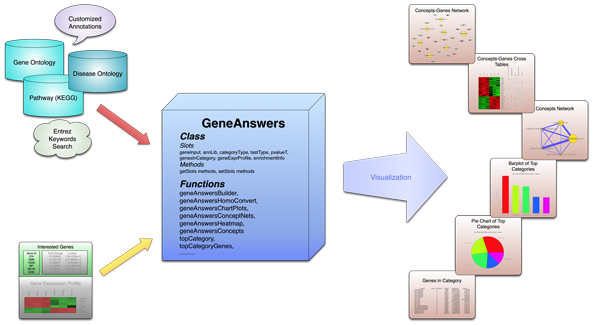
\includegraphics{flowchart.png}}
\caption{Flow chart of GeneAnswers}
\label{conceptgeneNetwork}
\end{figure}
\section{Data preprocessing}

First of all, load the \Rpackage{GeneAnswers} package.
\begin{Schunk}
\begin{Sinput}
> library(GeneAnswers)
\end{Sinput}
\end{Schunk}

\subsection{Build a GeneAnswers instance}
The key point of \Rpackage{GeneAnswers} package is to build a GeneAnswers instance. The essential input for \Rpackage{GeneAnswers} is an Entrez gene IDs vector (a character vector). However, if users have any interested values associated with genes, these values can also be as optional inputs. In this case,  the input, geneInput, could be a matrix or a dataframe. The first column is always for Entrez gene IDs. Other columns are used to store those interested values. Rownames for the matrix or dataframe are not necessary, but colnames are recommended for further usage. We use two internal datasets, one is from human and another is from mouse, as examples to show how to implement \Rpackage{GeneAnswers} package. The human and mouse datasets coming with the \Rpackage{GeneAnswers} package are  from human and mouse Illumina beadarray experiments. Each dataset contains two dataframes. For example, humanGeneInput is a dataframe  containing Entrez gene IDs with fold changes and p values, while the data frame, humanExpr, includes two types, control and treatment, of gene expression profile of the genes in humanGeneInput.

\begin{Schunk}
\begin{Sinput}
> data('humanGeneInput')
> data('humanExpr')
> ## build a GeneAnswers instance with statistical test based on biological process of GO and saved example data.
> x <- geneAnswersBuilder(humanGeneInput, 'org.Hs.eg.db', categoryType='GO.BP', testType='hyperG', pvalueT=0.1, geneExpressionProfile=humanExpr)
\end{Sinput}
\begin{Soutput}
[1] "geneInput has built in ..."
[1] "annLib and categoryType have built in ..."
[1] "genesInCategory has built in ..."
[1] "Enrichment test is only performed based on annotated genes"
[1] "testType, pvalueT and enrichmentInfo have built in ..."
[1] "geneExpressionProfile has been built in ..."
[1] "GeneAnswers instance has been successfully generated!"
\end{Soutput}
\begin{Sinput}
> class(x)
\end{Sinput}
\begin{Soutput}
[1] "GeneAnswers"
attr(,"package")
[1] "GeneAnswers"
\end{Soutput}
\begin{Sinput}
> ## build a GeneAnswers instance with statistical test based on KEGG and saved example data. 
> y <- geneAnswersBuilder(humanGeneInput, 'org.Hs.eg.db', categoryType='KEGG', testType='hyperG', pvalueT=0.1, geneExpressionProfile=humanExpr, verbose=FALSE)
\end{Sinput}
\begin{Soutput}
[1] "GeneAnswers instance has been successfully generated!"
\end{Soutput}
\begin{Sinput}
> ## build a GeneAnswers instance with statistical test based on DOLite and saved example data.
> z <- geneAnswersBuilder(humanGeneInput, 'org.Hs.eg.db', categoryType='DOLite', testType='hyperG', pvalueT=0.1, geneExpressionProfile=humanExpr, verbose=FALSE)
\end{Sinput}
\begin{Soutput}
[1] "GeneAnswers instance has been successfully generated!"
\end{Soutput}
\begin{Sinput}
> w <- geneAnswersBuilder(humanGeneInput, 'org.Hs.eg.db', categoryType='GO.BP', testType='hyperG', pvalueT=0.1, FDR.correct=TRUE, geneExpressionProfile=humanExpr, level=2, verbose=FALSE) 
\end{Sinput}
\begin{Soutput}
[1] "GeneAnswers instance has been successfully generated!"
\end{Soutput}
\end{Schunk}

We have four GeneAnswers objects, x, y, z and w, containing the statistical test of biological process of GO, KEGG, DOLite and GO (The first two level nodes are removed), respectively. For Gene Ontology, sometimes, users think some nodes are too general and not very relative to their interests. So we provide parameter {\it level} to determine how many top levels of GO nodes are removed. The instances have included the relationship between given genes and specified categories.

\Rpackage{GeneAnswers} package also provides a function {\it searchEntrez} to retrieve Entrez genes for given keywords by Entrez XML query. National Center for Biotechnology Information (NCBI) provides many powerful online query systems. One of them is Entrez Programming Utilities (eUtils). Users can query NCBI databases by simple keywords logical operations based on XML protocol. This is very helpful to find potential or interested biological functions or pathways. Hence, the retrieved information can be considered as a customized annotation library to test whether the given genes are relative to interested keywords. Here is a case to build a customized GeneAnswers instance.
\begin{Schunk}
\begin{Sinput}
> keywordsList <- list(Apoptosis=c('apoptosis'), CellAdhesion=c('cell adhesion'))
> entrezIDList <- searchEntrez(keywordsList) 
\end{Sinput}
\begin{Soutput}
[1] "search link: http://eutils.ncbi.nlm.nih.gov/entrez/eutils/esearch.fcgi?db=gene&term=apoptosis+AND+Homo+sapiens%5borganism%5d&retmode=xml&retmax=500000"
[1] "search link: http://eutils.ncbi.nlm.nih.gov/entrez/eutils/esearch.fcgi?db=gene&term=%22cell%20adhesion%22+AND+Homo+sapiens%5borganism%5d&retmode=xml&retmax=500000"
\end{Soutput}
\begin{Sinput}
> q <- geneAnswersBuilder(humanGeneInput, entrezIDList, testType='hyperG', totalGeneNumber = 45384, pvalueT=0.1, geneExpressionProfile=humanExpr, verbose=FALSE)
\end{Sinput}
\begin{Soutput}
[1] "GeneAnswers instance has been successfully generated!"
\end{Soutput}
\begin{Sinput}
> class(q)
\end{Sinput}
\begin{Soutput}
[1] "GeneAnswers"
attr(,"package")
[1] "GeneAnswers"
\end{Soutput}
\begin{Sinput}
> getAnnLib(q)
\end{Sinput}
\begin{Soutput}
NULL
\end{Soutput}
\begin{Sinput}
> getCategoryType(q)
\end{Sinput}
\begin{Soutput}
[1] "User defined"
\end{Soutput}
\end{Schunk}

Customized GeneAnswers instances have NULL at annLib slot and "User defiend" in categoryType slot.
 
\subsection{Visulization}
Besides barplot and pie chart, \Rpackage{GeneAnswers} package can generate a network (concept-gene network)  show how genes are connected to specified categories as well as general barplot and piechart. Function {\it GeneAnswersConceptNet} can generate a common R canvas or tcl/tk interactive canvas to draw the network by calling  \Rpackage{igraph}. Genes are presented as red nodes, if specified values are positive, and the gene nodes are green with negative values. The category nodes are yellow nodes, the sizes are relative to user-specified values. Currently, if function {\t GeneAnswersBuilder} successfully returns a GeneAnswers instance, the genes are represented as entrez IDs and categories are also category IDs. User can map them to gene symbols and categories terms by function {\it GeneAnswersReadable}. Function {\it GeneAnswersReadable} reads slot {\it annLib} to map Entrez IDs to gene symbols, so make sure slot {\it annLib} is correct before mapping.

\begin{Schunk}
\begin{Sinput}
> ## mapping gene IDs and category IDs to gene symbols and category terms
> xx <- geneAnswersReadable(x)
\end{Sinput}
\begin{Soutput}
[1] "Mapping geneInput ..."
[1] "Mapping genesInCategory ..."
[1] "Mapping enrichmentInfo rownames ..."
[1] "Mapping geneExprProfile rownames ..."
\end{Soutput}
\begin{Sinput}
> yy <- geneAnswersReadable(y, verbose=FALSE)
> zz <- geneAnswersReadable(z, verbose=FALSE)
> ww <- geneAnswersReadable(w, verbose=FALSE)
> q <- setAnnLib(q, 'org.Hs.eg.db')
> qq <- geneAnswersReadable(q, catTerm=FALSE) 
\end{Sinput}
\begin{Soutput}
[1] "Mapping geneInput ..."
[1] "Mapping genesInCategory ..."
[1] "Mapping geneExprProfile rownames ..."
\end{Soutput}
\end{Schunk}

Since function {\it geneAnswersReadable} implements mapping based on annotation database  in slot annLib, we assign 'org.Hs.eg.db' to customized GeneAnswers instance annLib slot at first for make it readable.

\begin{Schunk}
\begin{Sinput}
> ## plot barplot and / or piechart
> geneAnswersChartPlots(xx, chartType='all')
\end{Sinput}
\end{Schunk}

\begin{figure}
\centering
\centering
\resizebox{1\textwidth}{!}{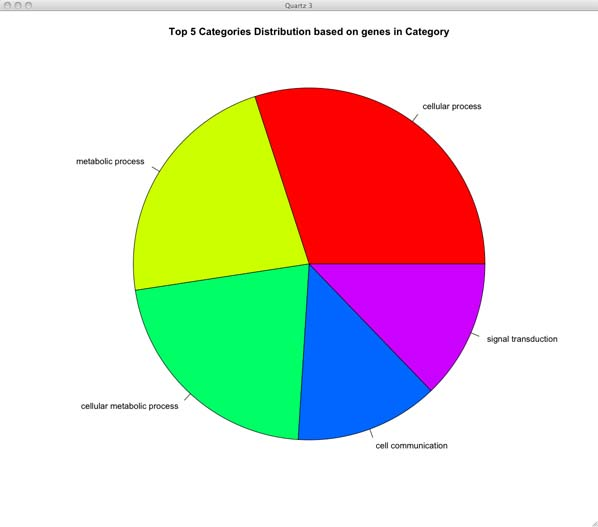
\includegraphics{piechart01.jpg}}
\caption{Screen shot of pie chart of top categories}
\label{pie chart of top categories}
\end{figure}

\begin{figure}
\centering
\centering
\resizebox{1\textwidth}{!}{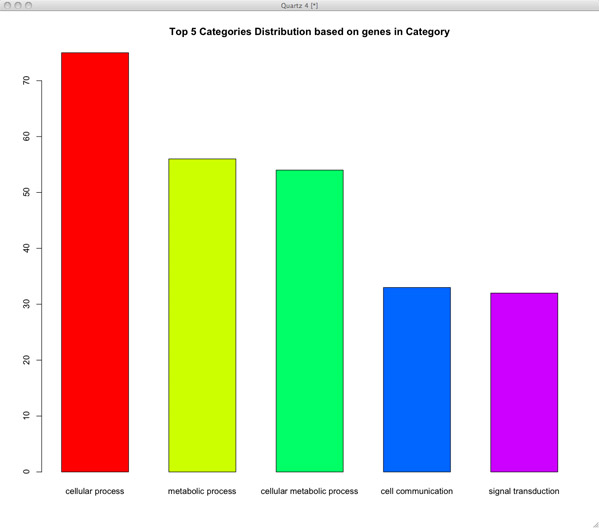
\includegraphics{barplot01.jpg}}
\caption{Screen shot of barplot of top categories}
\label{barplot of top categories}
\end{figure}   

The nodes could be represented by different colors for different specified values, like fold change. In this case, overexpressed genes are represented as red nodes while green dots stand for underexpressed genes. If the node is more red, which means its fold change is larger. It's same for green nodes, but different direction. 
\begin{Schunk}
\begin{Sinput}
> ## plot interactive concept-gene network
> geneAnswersConceptNet(xx, colorValueColumn='foldChange', centroidSize='pvalue', output='interactive')
\end{Sinput}
\end{Schunk}

\begin{figure}
\centering
\centering
\resizebox{1\textwidth}{!}{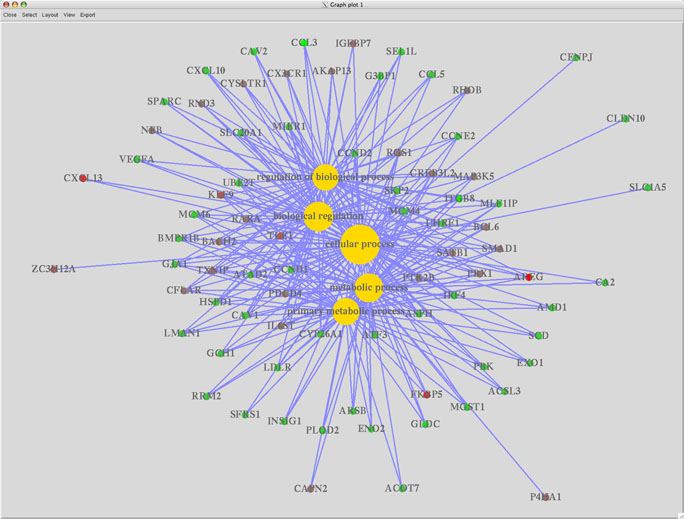
\includegraphics{conceptNet01a.jpg}}
\caption{Screen shot of concept-gene network}
\label{conceptgeneNetwork}
\end{figure}

The top 5 categories might not be very specific. Users might get a  tree view to see relative category terms by calling function geneAnswersConceptRelationif the category has an ontology structure. The size of nodes is proportional to number of genes in these GO categories. The color of nodes stand for how relative the given genes are to the GO categories. More red, more relative. The given GO categories are yellow framed dots with dark purple edges connetions.
\begin{Schunk}
\begin{Sinput}
> ## plot interactive go structure network
> geneAnswersConceptRelation(x, direction='both', netMode='connection', catTerm=TRUE, catID=TRUE, nameLength=15) 
\end{Sinput}
\end{Schunk}

\begin{figure}
\centering
\centering
\resizebox{1\textwidth}{!}{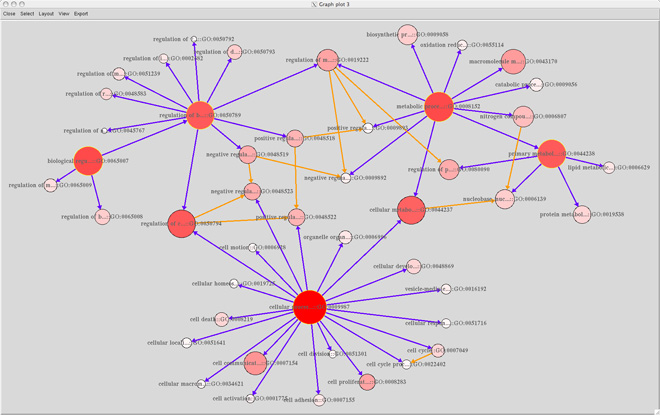
\includegraphics{gostrt.jpg}}
\caption{Screen shot of go structure network}
\label{conceptgeneNetwork}
\end{figure}

Also the new version GeneAnswers integrates gene or protein interaction database from NCBI. The following case is a typical one to show interaction information could be included in basic concepts-genes network.
\begin{Schunk}
\begin{Sinput}
> ## plot interactive concept-gene network
> geneAnswersConceptNet(x, color='foldChange', geneLayer=5, output='interactive', showCats=c("GO:0009611", "GO:0043933", "GO:0045622"), catTerm=TRUE, geneSymbol=TRUE, catID=TRUE)
\end{Sinput}
\end{Schunk}

\begin{figure}
\centering
\centering
\resizebox{1\textwidth}{!}{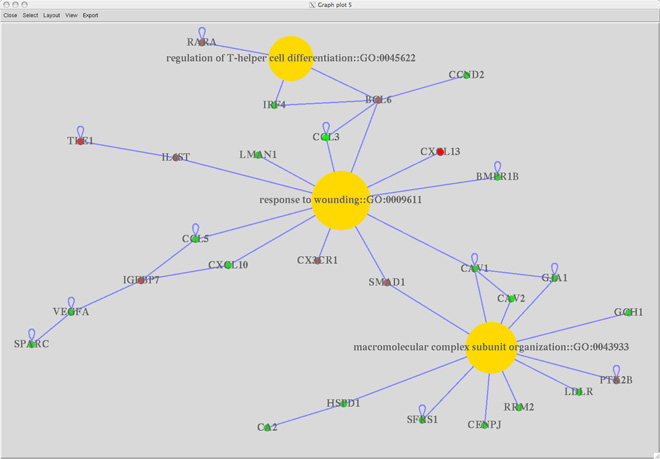
\includegraphics{conceptNet07.jpg}}
\caption{Screen shot of concept-gene network}
\label{conceptgeneNetwork}
\end{figure}


This function can also be used to show how the given genes interact with each other. For example, for the given genes in the GeneAnswers instance, x, users can use the following command to show gene '444','3638', '5087' and '55835' interact with each other and other genes in the given geneInput of x.
\begin{Schunk}
\begin{Sinput}
> ## plot the given gene interaction
> buildNet(c('444','3638', '5087','55835'), idType='GeneInteraction', layers=2, filterGraphIDs=getGeneInput(x)[,1], filterLayer=2, netMode='connection')
\end{Sinput}
\end{Schunk}

\begin{figure}
\centering
\centering
\resizebox{1\textwidth}{!}{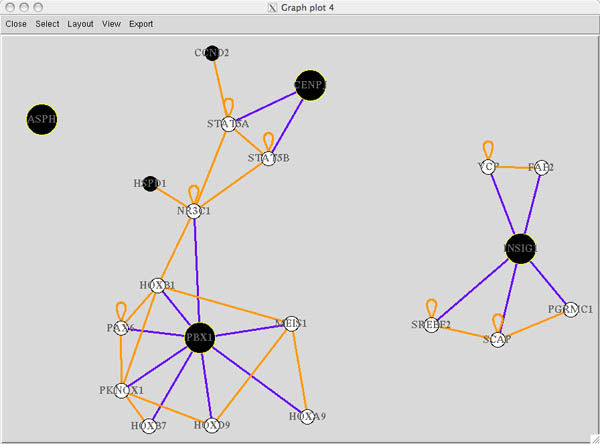
\includegraphics{geneInteraction01.jpg}}
\caption{Screen shot of the given gene interaction network}
\label{geneInteractionNetwork}
\end{figure}

In this case, large black dots with yellow frame stand for the 4 given genes. They also connect to other genes by dark-blue-purple edges. Small black dots represent the other genes from getGeneInput(x). Small white dots are genes that are not in the genes from getGeneInput(x), but interact with these genes. 

If there are some certain values associate with genes in geneInput of x, like the example data, you can represent any one column by colors. For example, if users want to show how genes interaction with gene expression information, the following command can show this:
\begin{Schunk}
\begin{Sinput}
> ## plot the given gene interaction
> buildNet(c('444','3638', '5087','55835'), idType='GeneInteraction', layers=2, filterGraphIDs=getGeneInput(x)[,1:2], filterLayer=2, netMode='connection')
\end{Sinput}
\end{Schunk}

\begin{figure}
\centering
\centering
\resizebox{1\textwidth}{!}{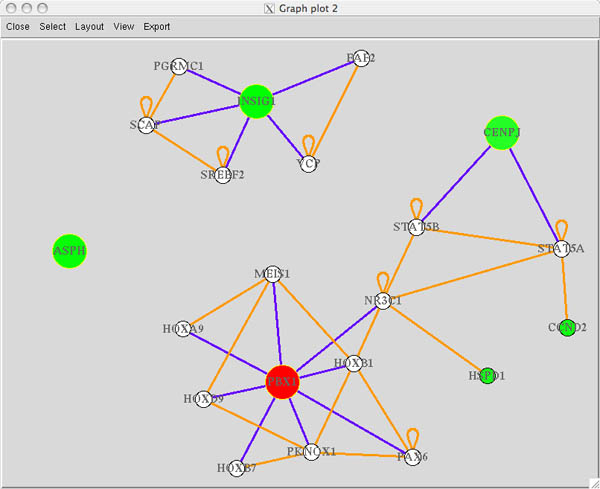
\includegraphics{geneInteraction02.jpg}}
\caption{Screen shot of the given gene interaction network with expression information}
\label{geneInteractionNetwork}
\end{figure}

The following one is based on expression p-values, we often use -log2 to transform p-values.
\begin{Schunk}
\begin{Sinput}
> ## plot the given gene interaction
> buildNet(c('444','3638', '5087','55835'), idType='GeneInteraction', layers=2, filterGraphIDs=cbind(getGeneInput(x)[,1], -log2(getGeneInput(x)[,3])), filterLayer=2, netMode='connection')
\end{Sinput}
\end{Schunk}

\begin{figure}
\centering
\centering
\resizebox{1\textwidth}{!}{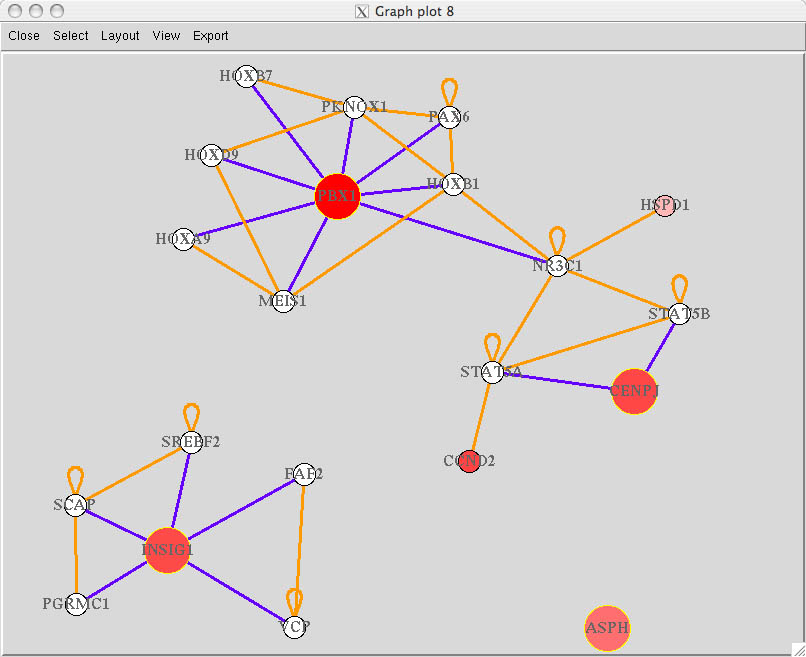
\includegraphics{geneInteraction03.jpg}}
\caption{Screen shot of the given gene interaction network with p-value information}
\label{geneInteractionNetwork}
\end{figure}

Users can also define customized color scheme and transfer it into 'buildNet' function by parameter 'colorMap'. Details are available in 'buildNet' manual page. If users want to have a overview for the interaction of all of the given genes from getGeneInput(x), the following command could be used:
\begin{Schunk}
\begin{Sinput}
> ## plot the given gene interaction
> buildNet(getGeneInput(x)[,1], idType='GeneInteraction', layers=2, filterGraphIDs=getGeneInput(x)[,1:2], filterLayer=2, netMode='connection')
\end{Sinput}
\end{Schunk}
\begin{figure}
\centering
\centering
\resizebox{1\textwidth}{!}{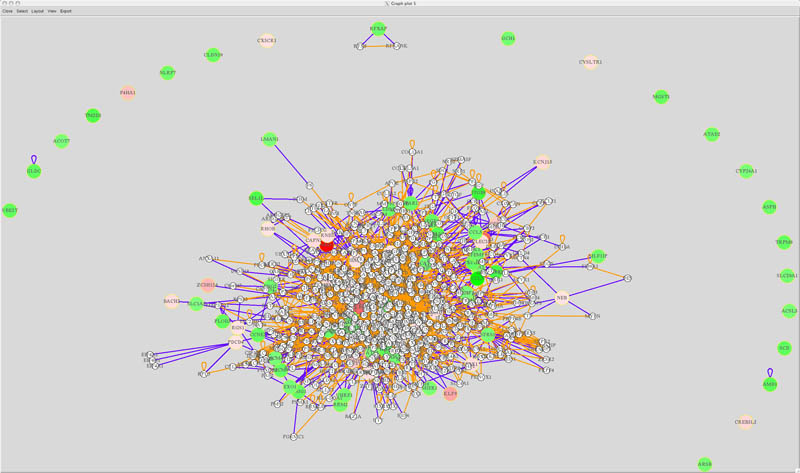
\includegraphics{geneInteraction04.jpg}}
\caption{Screen shot of all of the given gene interaction network with expression information}
\label{geneInteractionNetwork}
\end{figure}


If there are a lot of genes, the network could be very complicated. We strongly recommend to use 'interactive' mode to show the network since it's easy to manually change layout. The default setting is 'interactive', but users can change it to 'fixed' for a small or simple network.


The following example is to show top 5 GO-gene network for the first 2 level GO nodes removal.
\begin{Schunk}
\begin{Sinput}
> ## plot Go-concept network for 2 level nodes removal
> geneAnswersConceptNet(ww, colorValueColumn='foldChange', centroidSize='pvalue', output='fixed')
\end{Sinput}
\end{Schunk}


\begin{figure}
\centering
\centering
\resizebox{1\textwidth}{!}{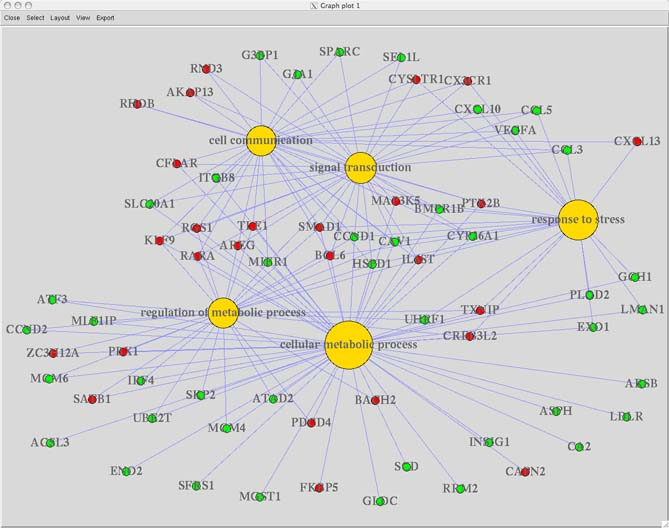
\includegraphics{conceptNet02.jpg}}
\caption{Screen shot of concept-gene network for top 2 GO level nodes removal}
\label{GO-genes network}
\end{figure}

Also, users can sort enrichment test information and plot it.
\begin{Schunk}
\begin{Sinput}
> ## sort enrichmentInfo dataframe by fdr adjusted p value
> xxx <- geneAnswersSort(xx, sortBy='correctedPvalue')